\documentclass[conference]{IEEEtran}
\IEEEoverridecommandlockouts
% IEEEtran standard template packages
\usepackage{cite}
\usepackage{amsmath,amssymb,amsfonts}
\usepackage{graphicx}
\usepackage{textcomp}
\usepackage{xcolor}
\usepackage{booktabs}
\usepackage{multirow}
\usepackage{url}
\usepackage{enumitem}
\usepackage{microtype}
\usepackage{tikz}
\usetikzlibrary{shapes.geometric, shapes.symbols, arrows.meta, positioning, fit, backgrounds, calc}

% Compact list and float spacing for strict 4-page target
\setlist[enumerate]{leftmargin=*,itemsep=0.5pt,topsep=1.5pt,parsep=0pt}
\setlist[itemize]{leftmargin=*,itemsep=0.5pt,topsep=1.5pt,parsep=0pt}
\setlength{\textfloatsep}{4pt plus 1pt minus 1pt}
\setlength{\floatsep}{4pt plus 1pt minus 1pt}
\setlength{\intextsep}{4pt plus 1pt minus 1pt}
\setlength{\abovecaptionskip}{2pt}
\setlength{\belowcaptionskip}{2pt}

\def\BibTeX{{\rm B\kern-.05em{\sc i\kern-.025em b}\kern-.08em
    T\kern-.1667em\lower.7ex\hbox{E}\kern-.125emX}}

\begin{document}

\title{Streams-and-Tables for Scalable Multi-Camera Object Tracking}

% =========================================================================
% AUTHOR BLOCK (ANONYMIZED FOR INITIAL DOUBLE-BLIND REVIEW PER NILES GUIDELINES)
% To activate full camera-ready author details, uncomment the section below.
% =========================================================================
\author{\IEEEauthorblockN{Anonymous Author(s)}
\IEEEauthorblockA{\textit{Affiliation Omitted for Double-Blind Review} \\
\textit{NILES 2026 Submission}}
}

%\author{
%\IEEEauthorblockN{Mahmoud Tayee}
%\IEEEauthorblockA{\textit{Faculty of Engineering and Applied Sciences} \\
%\textit{Nile University}, Giza, Egypt \\
%m.mostafa2118@nu.edu.eg}
%\and
%\IEEEauthorblockN{Ahmed Awad}
%\IEEEauthorblockA{\textit{Faculty of Computers and AI, Cairo University}, Egypt \\
%\textit{The British University in Dubai}, Dubai, UAE \\
%a.gaafar@fci-cu.edu.eg}
%}

\maketitle

\begin{abstract}
Multi-camera object tracking (MCOT) systems are traditionally constructed as monolithic computer-vision pipelines, causing combinatorial candidate explosions across non-adjacent cameras, burying identity state in program variables, and requiring hard restarts when camera network topology changes. We argue these limitations are architectural rather than algorithmic, and present a relational \emph{streams-and-tables} architecture for MCOT realized on an embeddable Complex Event Processing (CEP) engine: detections flow as append-only streams, identities and topology are queryable relational tables, and cross-camera association is a continuous topology-aware stream join. Evaluated on the Woven WTS and 9-camera NVIDIA SmartSpaces datasets, our system preserves exact functional parity with batch baselines while delivering a \textbf{9.8$\times$} speedup (\textbf{12.0$\times$} in representative selection, \textbf{9.5$\times$} in clustering) and a \textbf{4.16$\times$} latency reduction, with live topology events enabling zero-downtime reconfiguration in 190--337~ms.
% CAMERA-READY ONLY: uncomment to add the source-code link after the review.
% Source code and reproduction instructions are available at \url{https://github.com/MahmoudMostafaTayee/STREAMTRACK}.
\end{abstract}

\begin{IEEEkeywords}
Stream Processing, Complex Event Processing, Multi-Camera Object Tracking, Streams and Tables, Reconfigurable Systems, Edge Computing.
\end{IEEEkeywords}

% -------------------------------------------------------------------------
\section{Introduction}
\label{sec:intro}
Multi-camera object tracking (MCOT) underpins critical smart city applications, including urban traffic monitoring, intelligent space surveillance, and public safety analytics~\cite{yoshida2024overlap,kim2024cluster,xie2024robust}. The core task is to assign a unique, continuous global identity ($ID_G$) to each physical object as it traverses a network of cameras $\mathcal{C} = \{c_1,\dots,c_m\}$. While single-camera tracking (SCT) within a single field of view (FoV) is well handled by frame-to-frame trackers~\cite{yoshida2024overlap}, cross-camera association---matching tracklets across distinct cameras despite lighting changes, viewpoint shifts, occlusions, and non-overlapping spatial gaps---dominates system computational cost and dictates operational scalability.

\subsection{Problem Statement and Systems Bottlenecks}
The computer vision community traditionally treats multi-camera tracking scalability as an \emph{algorithmic} challenge (tighter Re-ID embeddings~\cite{ye2021deep} or heavier graph clustering heuristics). However, deploying MCOT in real-world environments raises three fundamental \emph{systems-level} architectural bottlenecks that academic vision benchmarks largely treat as implementation details:
\begin{enumerate}
    \item \textbf{Combinatorial Candidate Explosion:} Naive cross-camera association evaluates all camera pairs, scaling as $\binom{m}{2} = O(m^2)$. Real-world networks are spatially sparse; most pairs never observe the same person simultaneously, yet monolithic pipelines re-evaluate distant pairs indiscriminately.
    \item \textbf{Opaque, Uninspectable State:} Global identity assignments depend on continuously evolving state (tracklet-to-global mappings, last-seen coordinates). In monolithic pipelines this state is buried in imperative variables, making it impossible to query or audit \emph{why} an assignment was made.
    \item \textbf{Brittle, Static Topology:} Camera networks undergo frequent changes: cameras are added, removed, or re-linked. When topology is hardcoded into pipeline logic, reconfiguration requires editing code and restarting the pipeline, destroying accumulated tracking state.
\end{enumerate}

\vspace{-0.5em}
\subsection{Proposed Paradigm: Streams and Tables}
We argue these operational vulnerabilities stem from \emph{monolithic software architecture} rather than vision-algorithm constraints. Drawing on the \emph{stream--table duality}~\cite{sax2018streams}, we propose a continuous stream-processing architecture for MCOT. Detections and tracklet updates arrive as append-only event \emph{streams}; global identities and camera topology are maintained as mutable, queryable relational \emph{tables}; and cross-camera association is formulated as continuous spatial joins over live topology relations. Realized on an embeddable CEP engine in a single process, high-dimensional appearance feature tensors are shared zero-copy in memory, isolating architectural speedups from runtime and language overheads.

\textbf{Contributions:} (1) A streams-and-tables re-architecting of MCOT as an operator graph over detection streams and relational state tables; (2) topology-aware candidate pruning cutting evaluations from $\binom{9}{2}=36$ to $6$ pairs (\textbf{4.16$\times$} latency reduction); (3) five-stage parity verification against a JVM batch baseline on Woven WTS, confirming 100\% Global ID parity with a \textbf{9.8$\times$} speedup; and (4) an event-driven control plane enabling zero-downtime reconfiguration in 190--337~ms with total state preservation.

% -------------------------------------------------------------------------
\section{Background and Related Work}
\label{sec:background}

\subsection{Multi-Camera People Tracking Baselines}
High-performing MCOT solutions catalysed by the AI City Challenge~\cite{yoshida2024overlap,kim2024cluster,xie2024robust,specker2024ocmctrack,yang2024online} focus predominantly on computer-vision heuristics. Yoshida et al.~\cite{yoshida2024overlap} proposed Overlap Suppression Clustering (OSC) for offline batch tracking, using degree centrality to resolve overlap anomalies and average-linkage hierarchical clustering (HAC) over pose keypoint confidence levels. Online entries like Kim et al.~\cite{kim2024cluster} (Cluster Self-Refinement) and Xie et al.~\cite{xie2024robust} employ periodic batch clustering windows or geometric projection constraints. However, these systems treat tracking as a monolithic pipeline, relying on periodic offline or semi-batch passes to rectify accumulated errors.

Industrial platforms like NVIDIA DeepStream~\cite{nvidia2024deepstream} and Metropolis~\cite{nvidia2025metropolis} provide containerized microservice execution, but association logic remains embedded in closed-source modules; state is not natively queryable via SQL, and topology updates require manual service redeployments.

\subsection{Stream--Table Duality and CEP Engine Selection}
Continuous Query Language (CQL) models~\cite{sax2018streams,DBLP:journals/vldb/ArasuBW06} unify streaming and relational data across four operator families:
\begin{itemize}
    \item \textbf{Stream-to-Relation (S2R):} Temporal sliding windows (\texttt{win:time}) capturing stream subsets into relations.
    \item \textbf{Relation-to-Relation (R2R):} Relational SQL queries over materialised state tables.
    \item \textbf{Stream/Relation-to-Relation (S/R2R):} Stream updates mutating persistent relational tables (upserts).
    \item \textbf{Relation-to-Stream (R2S):} Timer-driven evictions emitting derived event streams.
\end{itemize}

While distributed engines (e.g., Apache Flink, Kafka Streams) excel at data-parallel key-value tasks, transferring high-dimensional appearance vectors across network sockets incurs severe RPC serialisation overhead. We select Esper~\cite{espertech2024}, a mature CEP engine providing full CQL semantics in an embeddable, single-process JVM runtime, enabling zero-copy sharing of feature vectors between vision kernels and relational state tables.

% -------------------------------------------------------------------------
\section{System Architecture}
\label{sec:architecture}

Our system decomposes MCOT execution into two decoupled planes: a \emph{Data Plane} executing continuous tracking operators and a \emph{Control Plane} managing live configuration relations, as illustrated in Fig.~\ref{fig:architecture}.

\begin{figure}[t!]
\centering
\resizebox{\linewidth}{!}{
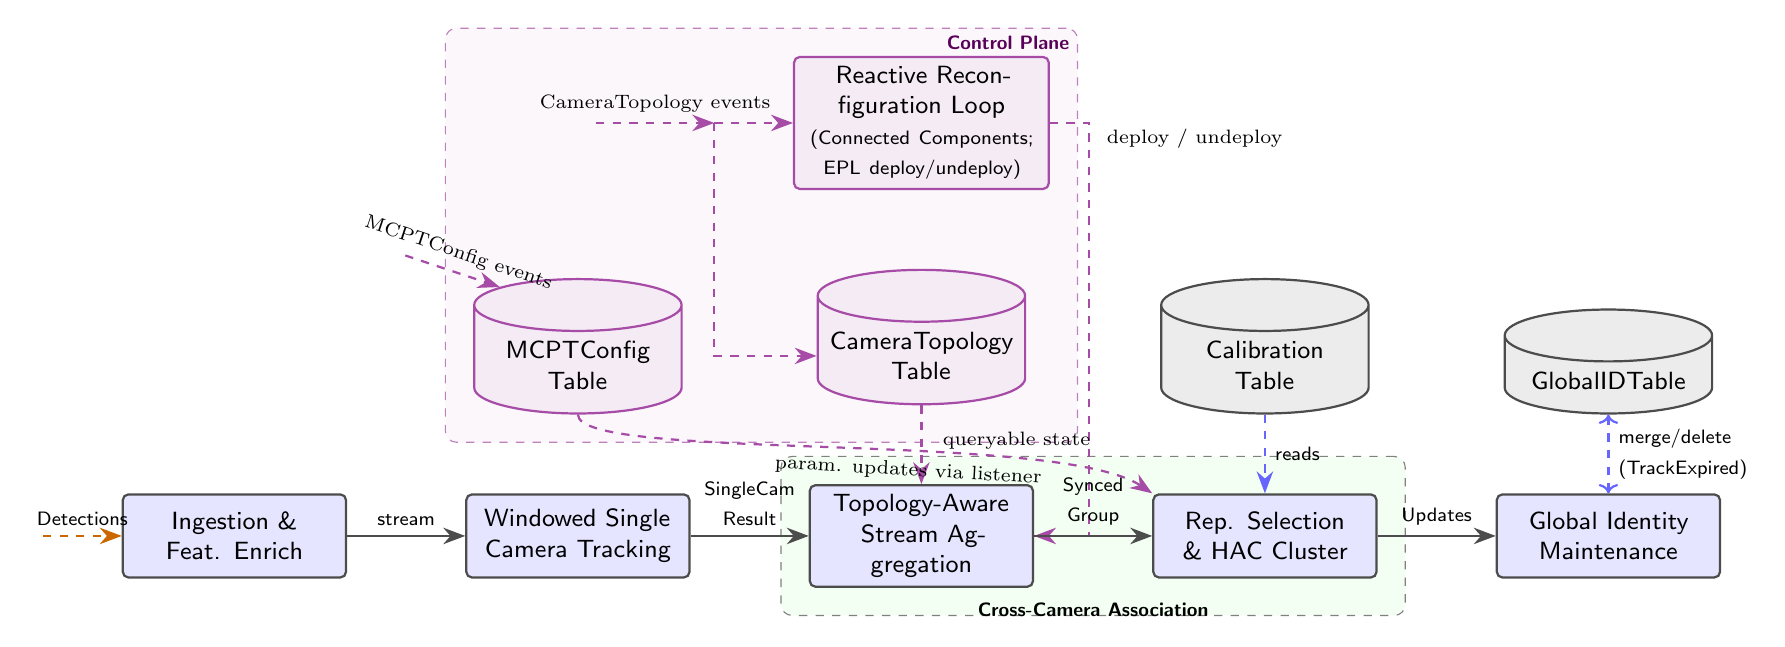
\begin{tikzpicture}[
    node distance=1.2cm and 1.5cm,
    font=\small\sffamily,
    block/.style={rectangle, draw=black!70, fill=blue!10, rounded corners=2pt, minimum height=3em, text width=2.6cm, align=center, thick},
    ctrlblock/.style={rectangle, draw=violet!70, fill=violet!8, rounded corners=2pt, minimum height=3em, text width=3.0cm, align=center, thick},
    table/.style={cylinder, shape border rotate=90, aspect=0.25, draw=black!70, fill=gray!15, text width=2.4cm, align=center, minimum height=3.5em, thick},
    ctrltable/.style={cylinder, shape border rotate=90, aspect=0.25, draw=violet!70, fill=violet!8, text width=2.4cm, align=center, minimum height=3.5em, thick},
    arrow/.style={-{Stealth[scale=1.2]}, thick, draw=black!70},
    stream/.style={-{Stealth[scale=1.2]}, thick, draw=orange!80!black, dashed},
    staterw/.style={-{Stealth[scale=1.2]}, thick, draw=blue!60, dashed},
    ctrl/.style={-{Stealth[scale=1.2]}, thick, draw=violet!70, dashed},
    group_box/.style={rectangle, draw=black!50, rounded corners=4pt, inner sep=10pt, dashed}
]
% ---------------- DATA PLANE ----------------
\node[block] (ingest) {Ingestion \& \\ Feat. Enrich};
\node[block, right=of ingest] (scpt) {Windowed Single \\ Camera Tracking};
\node[block, right=of scpt] (join) {Topology-Aware \\ Stream Aggregation};
\node[block, right=of join] (mcpt) {Rep. Selection \\ \& HAC Cluster};
\node[block, right=of mcpt] (global) {Global Identity \\ Maintenance};
\node[table, above=1.0cm of mcpt] (calibration) {Calibration\\Table};
\node[table, above=1.0cm of global] (globaltable) {GlobalIDTable};
% ---------------- CONTROL PLANE ----------------
\node[ctrltable, above=1.0cm of join] (topology) {CameraTopology\\Table};
\node[ctrltable, above=1.0cm of scpt] (configtable) {MCPTConfig\\Table};
\node[ctrlblock, above=1.0cm of topology] (reconfig) {Reactive Reconfiguration Loop\\ \scriptsize (Connected Components; EPL deploy/undeploy)};
% control event streams entering from the left
\draw[ctrl] ($ (configtable.north west) + (-1.2,0.4) $) -- node[above, font=\scriptsize, sloped] {MCPTConfig events} (configtable.north west);
% CameraTopology events: split to two parallel targets
\draw[ctrl] ($ (reconfig.west) + (-2.5,0) $) -- node[above, font=\scriptsize] {CameraTopology events} ($ (reconfig.west) + (-1.0,0) $);
\draw[ctrl] ($ (reconfig.west) + (-1.0,0) $) -- (reconfig.west);
\draw[ctrl] ($ (reconfig.west) + (-1.0,0) $) |- (topology.west);
% control wiring
\path (reconfig.east) ++(0.5,0) coordinate (rjoin);
\draw[ctrl] (reconfig.east) -- (rjoin) |- (join.east);
\path (rjoin) ++(0.1,-0.2) node[right, font=\scriptsize] {deploy / undeploy};
% table read by aggregation queries
\path (topology.south) ++(0,-0.45) coordinate (tjoin);
\draw[ctrl] (topology.south) -- (tjoin) -| (join.north);
\path (tjoin) ++(0.15,0) node[right, font=\scriptsize] {queryable state};
\draw[ctrl] (configtable.south) .. controls +(0,-0.6) and +(-1.2,0.8) .. node[below, font=\scriptsize, sloped, pos=0.6] {param. updates via listener} (mcpt.north west);
% ---------------- Data-plane arrows ----------------
\draw[stream] ($ (ingest.west) - (1cm,0) $) -- node[above] {\scriptsize Detections} (ingest.west);
\draw[arrow] (ingest) -- node[above] {\scriptsize stream} (scpt);
\draw[arrow] (scpt) -- node[above, align=center] {\scriptsize SingleCam\\ \scriptsize Result} (join);
\draw[arrow] (join) -- node[above, align=center] {\scriptsize Synced\\ \scriptsize Group} (mcpt);
\draw[arrow] (mcpt) -- node[above] {\scriptsize Updates} (global);
\draw[staterw] (calibration) -- node[right] {\scriptsize reads} (mcpt);
\draw[staterw, <->] (globaltable) -- node[right, align=left] {\scriptsize merge/delete\\ \scriptsize (TrackExpired)} (global);
% ---------------- Group backgrounds ----------------
\begin{scope}[on background layer]
    \node[group_box, fit=(join) (mcpt), fill=green!5,
      label={[anchor=base, inner sep=1pt, font=\scriptsize\bfseries\sffamily]below:Cross-Camera Association}] {};
    \node[group_box, draw=violet!50, fit=(reconfig) (configtable) (topology), fill=violet!3,
      label={[anchor=north east, inner sep=3pt, font=\scriptsize\bfseries\sffamily, text=violet!70!black]north east:Control Plane}] {};
\end{scope}
\end{tikzpicture}
}
\caption{Proposed operator graph: the \emph{data plane} processes detections through single-camera tracking, topology-aware aggregation, and HAC clustering, with \texttt{CalibrationTable} and \texttt{GlobalIDTable} as relational state; the \emph{control plane} (violet) upserts \texttt{CameraTopology} and \texttt{MCPTConfig} events into control tables while a reactive loop deploys/undeploys association queries at runtime with zero downtime.}
\label{fig:architecture}
\end{figure}

\subsection{Data Plane: Incremental Stream Processing}
1) \textbf{Ingestion and Intra-Camera Overlap Suppression (S2S):} Per-camera detection streams undergo Non-Maximum Suppression (NMS) at ingestion to eliminate overlapping duplicate bounding boxes; this differs from cross-camera field-of-view (FoV) overlap, a spatial relation modeled in \texttt{CameraTopologyTable}.

2) \textbf{Windowed Single-Camera Tracking (S2R):} Local frame detections are grouped into tracklets over a 3-second sliding window (90 frames at 30~fps, \texttt{win:length\_batch(90)}), emitting structured single-camera result events.

3) \textbf{Representative Feature Selection (S/R2S):} For each tracklet, the system queries \texttt{CalibrationTable} to select top-$k$ observations by anatomical keypoint confidence and embedding temporal stability; visibility filters reject occluded boxes before Re-ID matching.

4) \textbf{Topology-Aware Aggregation and HAC Clustering (S2R $\to$ R2S):} Tracklets in the same spatial neighbourhood are window-synchronized and joined; a windowed Hierarchical Agglomerative Clustering (HAC) kernel then clusters appearance embeddings into global identity candidates.

5) \textbf{Global Identity Maintenance (S/R2R and R2S):} Mappings are materialised in a persistent \texttt{GlobalIDTable}; cluster events trigger atomic \texttt{on-merge} upserts of last-seen timestamps, while timer queries evict stale tracks (unseen $>120$~s) via \texttt{TrackExpiredEvent} (R2S) before an R2R deletion garbage-collects heavy feature tensors.

\subsection{Cross-Camera Candidate Pruning and Join Planning}
Naive all-pairs matching across $m$ cameras evaluates $\binom{m}{2}$ pairs. When the network is partitioned into $k$ spatial topology groups of sizes $n_1, \dots, n_k$ ($\sum n_i = m$), the required candidate evaluations drop sharply to $\sum_{i=1}^{k} \binom{n_i}{2}$.

For our 9-camera deployment (Fig.~\ref{fig:topology_map}) partitioned into four spatial groups ($\{[02,17], [01,11], [19,27], [21,25,30]\}$), candidate evaluations decrease from $\binom{9}{2} = 36$ to $1+1+1+3 = 6$ camera pairs---a \textbf{6$\times$ candidate search space reduction}. Physical execution bakes these topology filters into query plans during compilation, avoiding per-tuple table probes on the hot path.

\begin{figure}[t!]
    \centering
    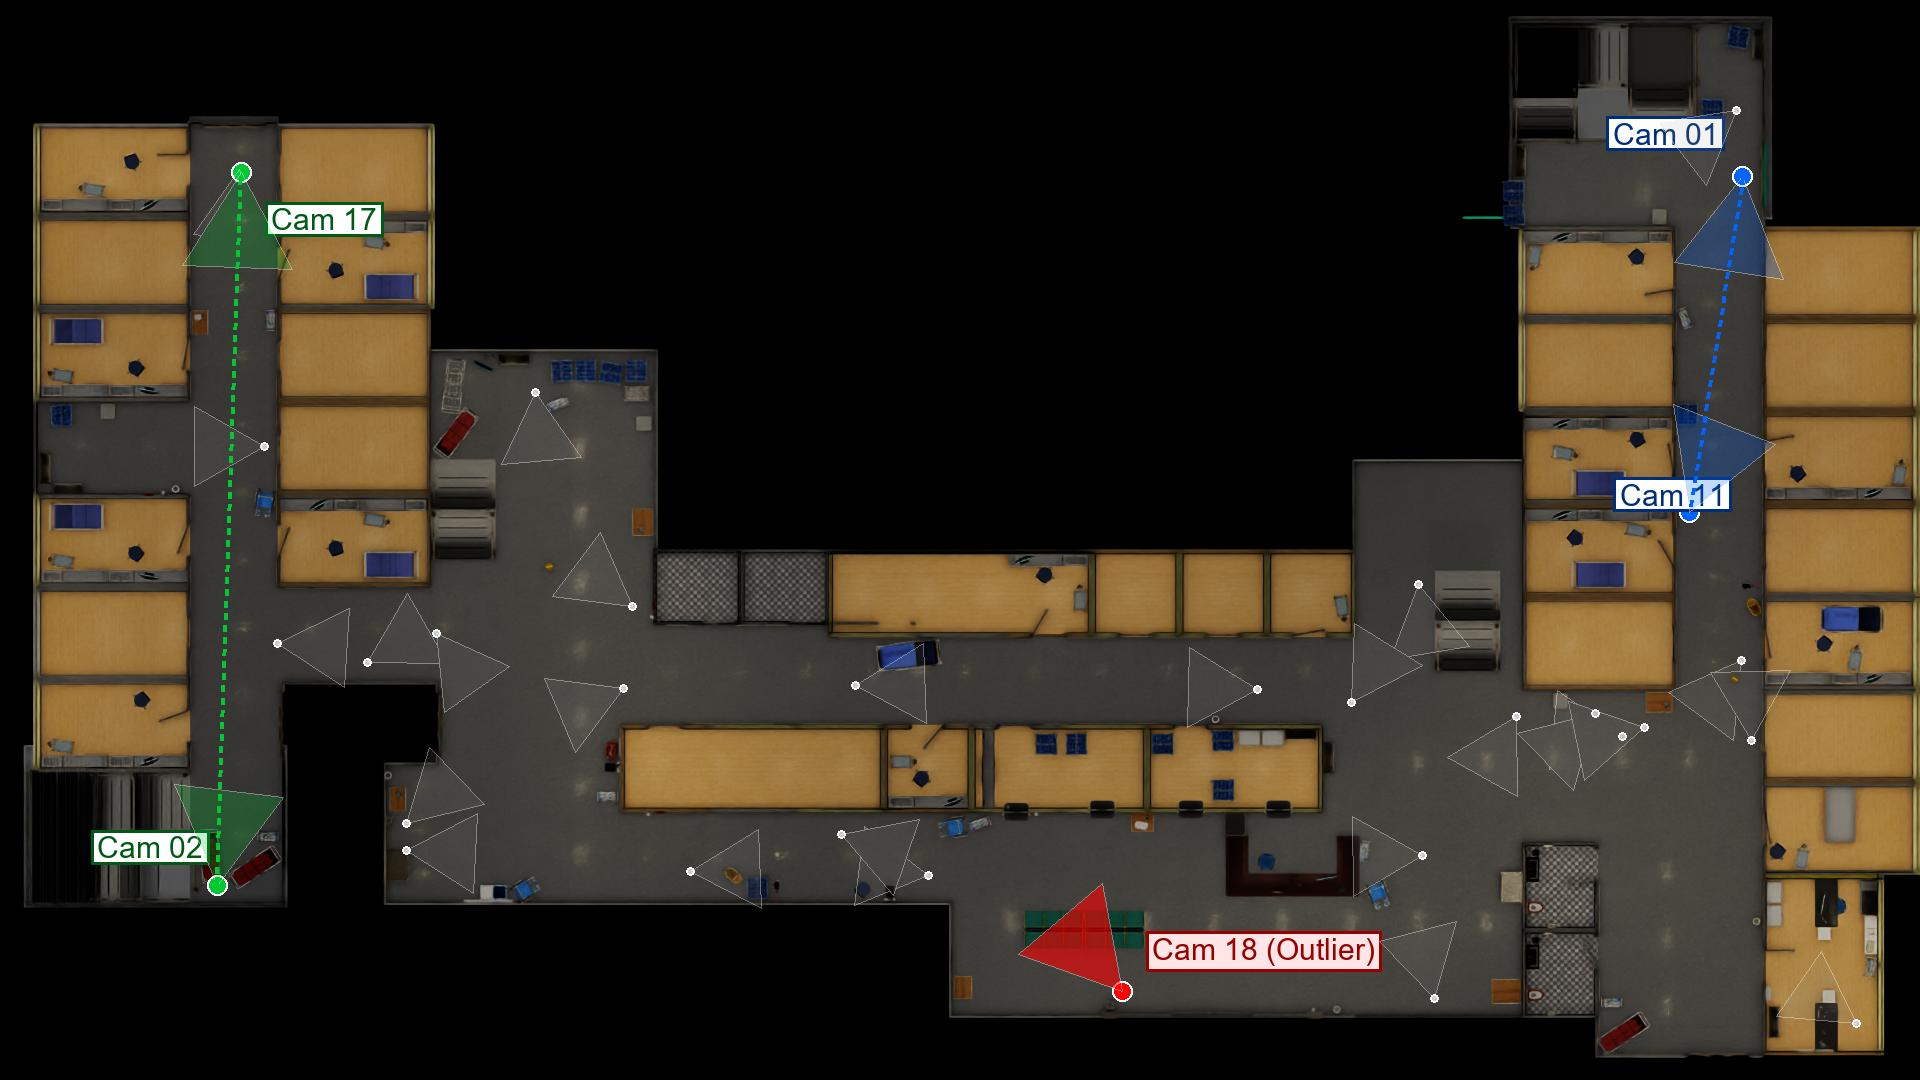
\includegraphics[width=1\linewidth]{Evidence/map_topology.png}
    \caption{Topological partitioning of the 9-camera NVIDIA SmartSpaces network into four spatial groups: Group 1 (blue: C02, C17), Group 2 (green: C01, C11), Group 3 (orange: C19, C27), and Group 4 (purple: C21, C25, C30).}
    \label{fig:topology_map}
\end{figure}

\subsection{Transitional Gating for Non-Overlapping Cameras}
To track objects across isolated, non-overlapping cameras without identity fragmentation, the topology relation maintains both overlapping edges ($E_{\text{overlap}}$) and directed transition edges ($E_{\text{transition}}$). During global association, candidate comparisons between historical tracks $T_H$ in \texttt{GlobalIDTable} and current cluster $C_{\text{curr}}$ are gated by:
\begin{equation}
\mathrm{ReIDAllowed}(T_H, C_{\mathrm{curr}}) = 
\begin{cases}
\text{True}, & \text{if } c_{\mathrm{last}} \in C_{\mathrm{curr}} \\
\text{True}, & \text{if } \exists c \in C_{\mathrm{curr}} \text{ s.t. } \\
             & (c_{\mathrm{last}}, c) \in E_{\mathrm{ovl}} \cup E_{\mathrm{trn}} \\
\text{False}, & \text{otherwise}
\end{cases}
\end{equation}
where $c_{\mathrm{last}} = \text{LastCam}(T_H)$, $E_{\mathrm{ovl}} = E_{\text{overlap}}$, and $E_{\mathrm{trn}} = E_{\text{transition}}$. This restricts candidate comparisons strictly to physically valid travel routes, preventing false matches across distant areas of the network.

\subsection{Control Plane: Reactive Reconfiguration Loop}
Camera topology is stored in a mutable \texttt{CameraTopologyTable}. When administrators stream \texttt{CameraTopology} update events (e.g., adding a link or camera outage), an \texttt{on-merge} query updates table state while a parallel listener triggers a Java controller (\texttt{reconcileDeployments()}) that recomputes connected components, undeploys obsolete aggregation queries, and compiles fresh EPL joins for the new groups---\textbf{zero-downtime reconfiguration} without restarts or state loss.

Similarly, tracking parameters (similarity threshold $\text{simTh}$, clustering radius $\epsilon_{\text{mcpt}}$) live in an \texttt{MCPTConfigTable} and are re-read on every window call.

% -------------------------------------------------------------------------
\section{Experimental Evaluation}
\label{sec:evaluation}

\subsection{Experimental Setup}
All experiments ran on an Intel Core i7-10610U CPU (4 cores, 8 threads, 1.80~GHz), 32~GB RAM, 64-bit Windows 11 Pro, OpenJDK 21 (JBR-21.0.8), with JVM heap capped at \texttt{-Xms256m -Xmx256m} to simulate resource-constrained edge gateways and Esper 9.0.0 as the CEP engine. Datasets: (1) Woven VisionAI WTS (Scene 2, 4 cameras)~\cite{kong2024wts} for parity and stage speedups; (2) NVIDIA SmartSpaces (9 cameras)~\cite{aicity2025track1} for topological pruning and live reconfiguration.

\subsection{RQ1: Five-Stage Implementation Parity and Speedup}
To verify that our re-engineering preserves accuracy, we conducted a \textbf{five-stage parity evaluation} against a JVM-native batch baseline. As the cited OSC pipeline~\cite{yoshida2024overlap} is Python, we ported it to this functionally equivalent JVM baseline, validated on identical inputs (ARI = NMI = 1.0000; similarity-matrix MAD $1.63\times10^{-8}$):
\begin{enumerate}
    \item \textbf{Numerical Parity:} Cosine matrices match across RAW, ZEROED, and REPLACED stages ($\text{MAD} = 1.63 \times 10^{-8}$; 98.37\% of RAW cells within $10^{-10}$, rising to 99.01\% after zeroing/replacement).
    \item \textbf{Structural Parity:} Adjusted Rand Index ($\text{ARI}$) and Normalized Mutual Information ($\text{NMI}$) achieve \textbf{1.0000} across all 175 tracklets (14/14 identity clusters match perfectly).
    \item \textbf{Post-Processing Parity:} Within-camera NMS and warp-merge fusion generate identical label assignments ($\text{ARI} = \text{NMI} = 1.0000$).
    \item \textbf{Topology Parity:} Inter-camera matrix converges to an identical $12\times 12$ shape.
    \item \textbf{Identity Parity:} Final global person identity assignments match with \textbf{100.00\% structural equivalence}.
\end{enumerate}

\begin{table}[t!]
\centering
\caption{Five-Stage Parity and Architectural Speedup (Woven WTS Dataset)}
\label{tab:performance_combined}
\resizebox{\linewidth}{!}{
\begin{tabular}{lrrrc}
\toprule
\textbf{Pipeline Stage} & \textbf{Batch (ms)} & \textbf{Streaming (ms)} & \textbf{Speedup} & \textbf{Parity Metric} \\
\midrule
Representative Selection & 10,235.16 & $34.06 \pm 36.52$ & \textbf{12.0$\times$} & Keypoint Exact \\
Clustering (HAC) & 20,366.55 & $86.16 \pm 68.86$ & \textbf{9.5$\times$} & ARI = NMI = 1.00 \\
Global ID Management & 521.00 & $3.13 \pm 1.97$ & \textbf{6.7$\times$} & 100\% Match \\
Matrix Zeroing & 6.09 & $0.03 \pm 0.04$ & \textbf{8.6$\times$} & MAD $= 0.99\times 10^{-8}$ \\
Re-ID Similarity Matrix & 65.08 & $3.67 \pm 8.28$ & Parity & MAD $= 1.63\times 10^{-8}$ \\
World Coord. Measure & 8.65 & $1.25 \pm 0.79$ & Parity & Exact Match \\
World Coord. Replace & 0.06 & $0.002 \pm 0.010$ & \textbf{1.0$\times$} & Exact Match \\
\midrule
\textbf{Total MCPT Processing} & \textbf{31,620.00} & \textbf{$129.27 \pm 92.49$} & \textbf{9.8$\times$} & \textbf{Global ID 100\%} \\
\bottomrule
\end{tabular}
}
\end{table}

\begin{figure}[t!]
    \centering
    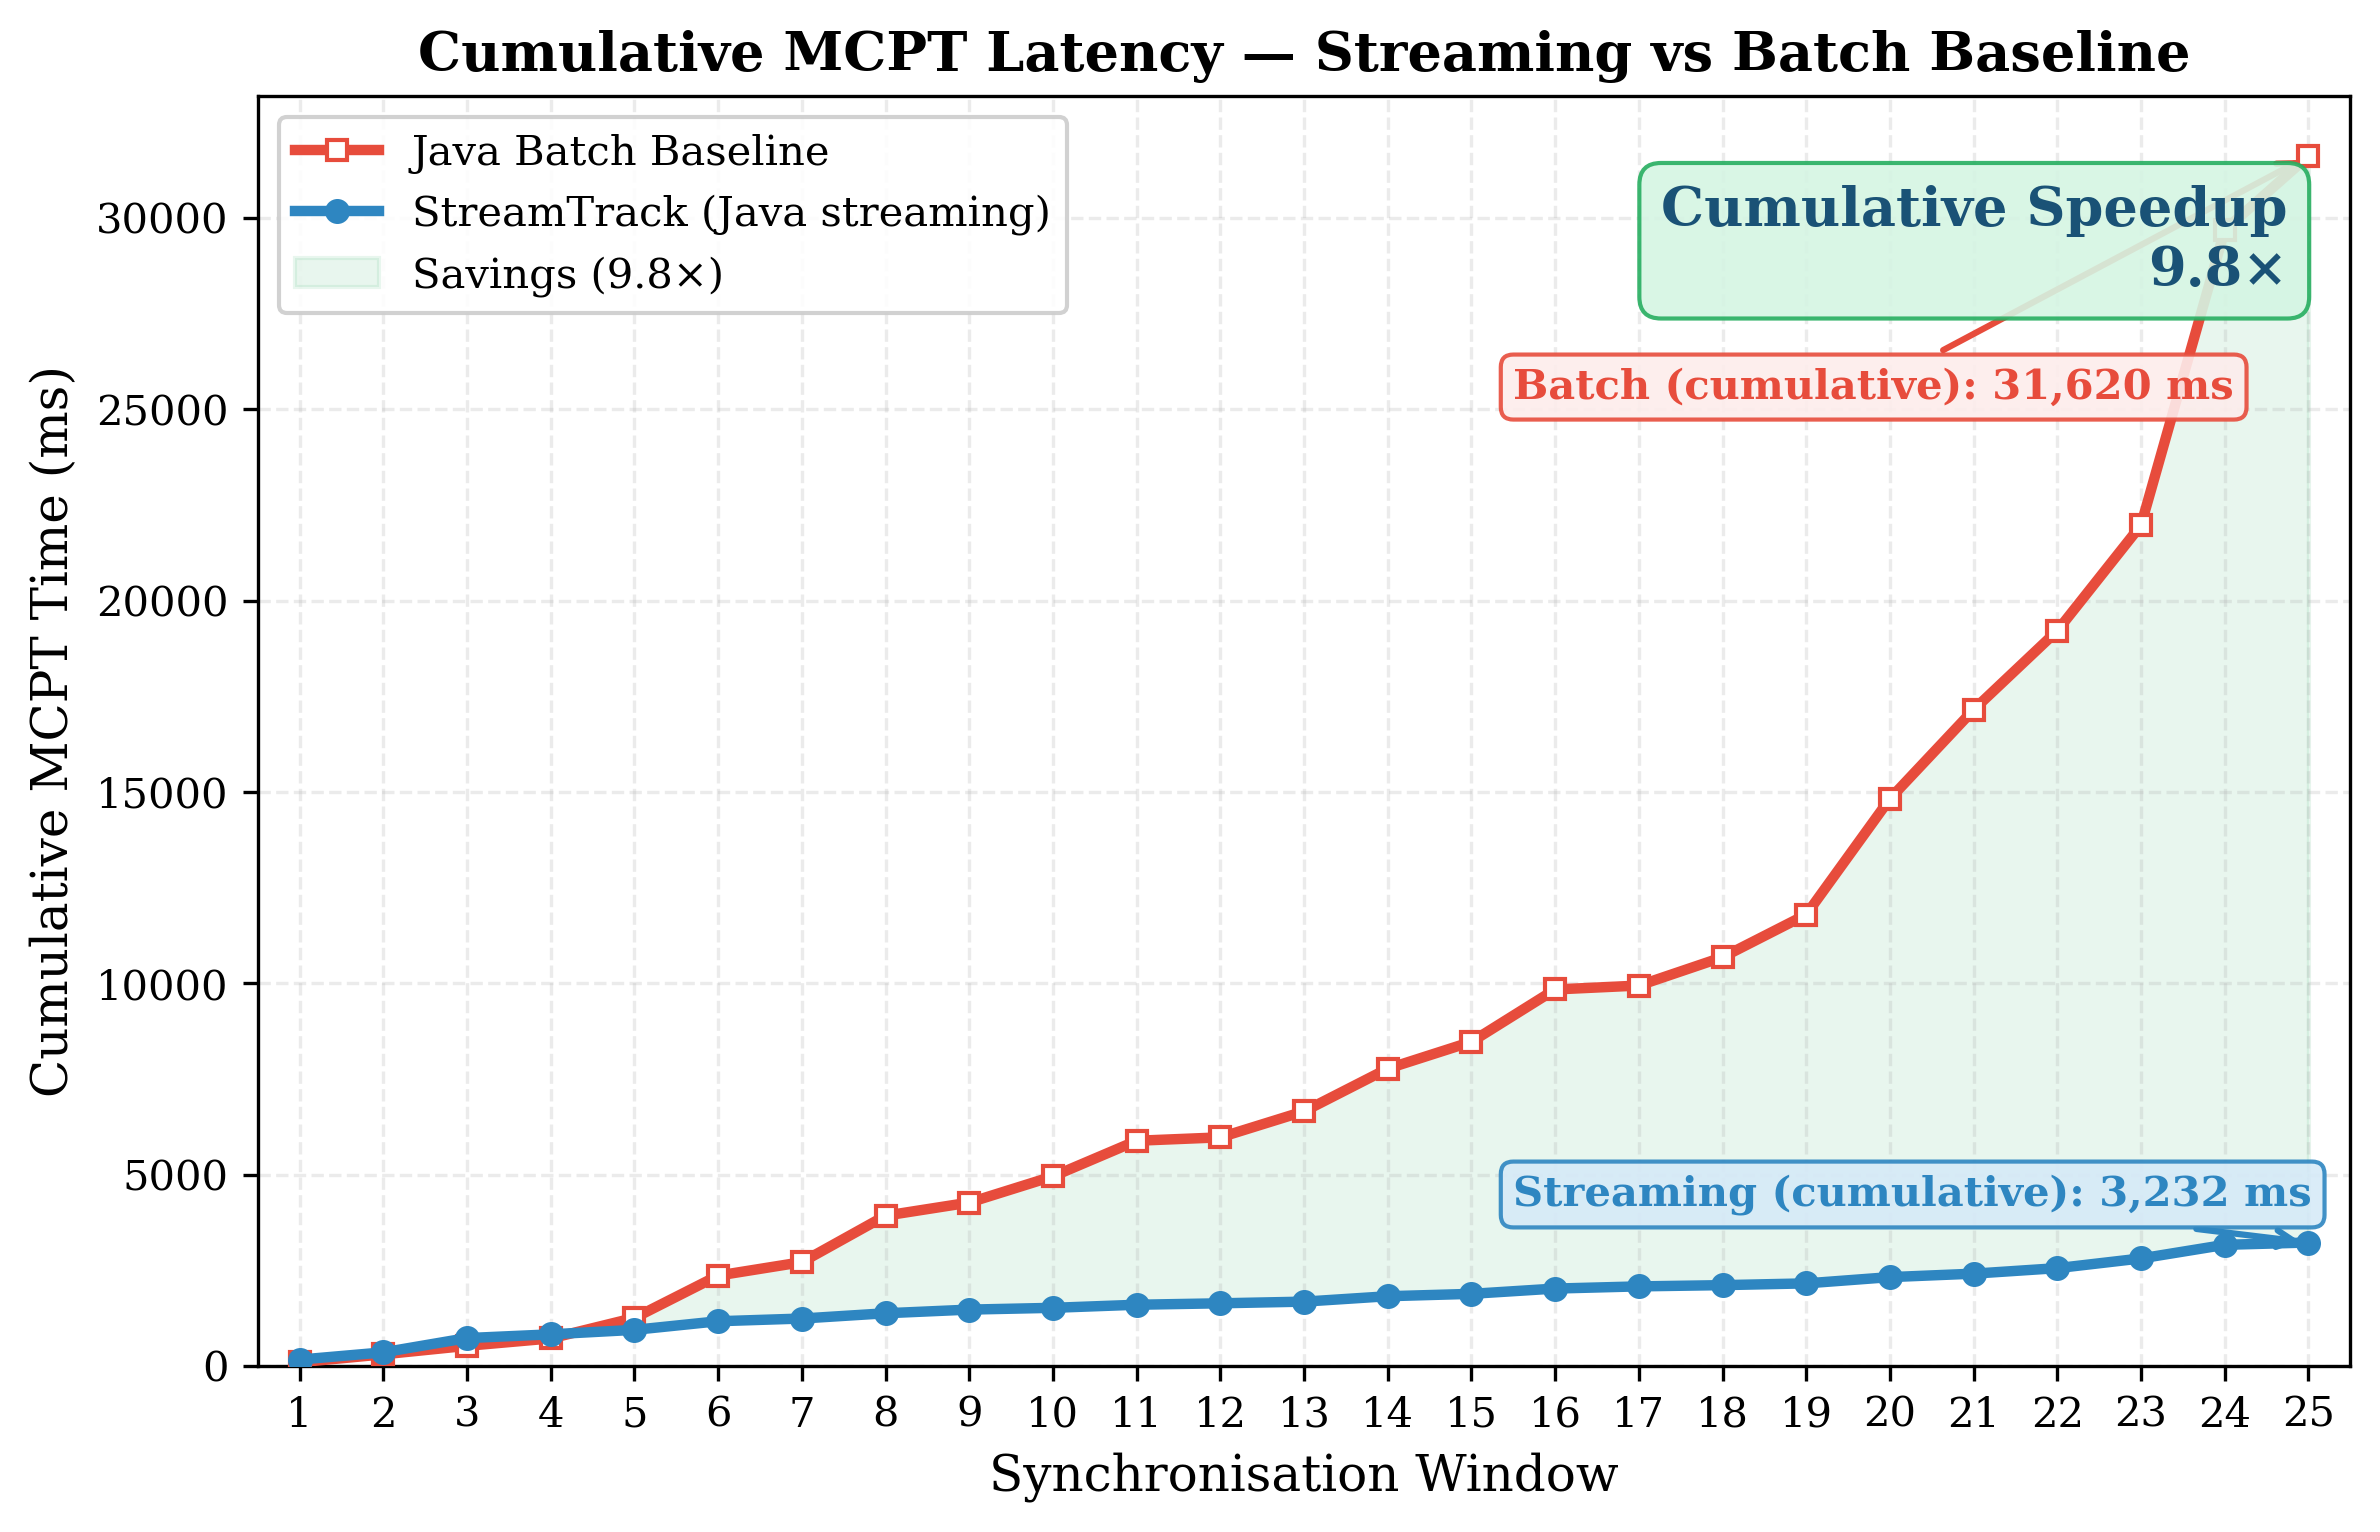
\includegraphics[width=1\linewidth]{Evidence/fig_cumulative_mcpt.png}
    \caption{Cumulative MCPT latency across 25 consecutive windows on the Woven WTS dataset (4 cameras). Incremental streaming achieves a \textbf{9.8$\times$} speedup over the batch baseline by eliminating redundant state recomputation.}
    \label{fig:cumulative_mcpt}
\end{figure}

The batch baseline re-reads and re-processes full historical feature archives from disk each window ($O(N^2)$ growth), requiring 31,620~ms total; our system maintains state incrementally in relational tables, reducing cumulative execution to 3,232~ms---a \textbf{9.8$\times$ end-to-end speedup} (Fig.~\ref{fig:cumulative_mcpt}), with \textbf{12.0$\times$} in representative selection and \textbf{9.5$\times$} in HAC clustering.

\subsection{RQ2: Clustering Operator Choice and Topological Optimization}
We benchmarked windowed HAC against specialized stream-clustering algorithms (CluStream~\cite{aggarwal2003framework} and ClusTree~\cite{kranen2011clustree} via MOA~\cite{bifet2010moa}). HAC achieves superior latency ($82.4$~ms) and 100\% identity precision for typical MCOT window sizes ($N=50$--$500$), whereas micro-cluster summaries in CluStream introduce high initialization overhead ($3,854.2$~ms) and blur fine-grained appearance features.

On the 9-camera NVIDIA SmartSpaces network (Table~\ref{tab:9camera_performance}), partitioning into 4 topological groups reduces average association latency from 41.96~ms to 10.10~ms (\textbf{4.16$\times$} with JVM JIT warm-up) and to 9.15~ms (\textbf{4.27$\times$} steady state).

\begin{table}[t!]
\centering
\caption{Topological Optimization Impact (NVIDIA SmartSpaces, 10 Runs)}
\label{tab:9camera_performance}
\resizebox{\linewidth}{!}{
\begin{tabular}{lccc}
\toprule
\textbf{Execution Mode} & \textbf{Global (1 Group)} & \textbf{Topology-Aware (4 Groups)} & \textbf{Speedup} \\
\midrule
Avg. Latency (inc. JIT warm-up) & $41.96 \pm 22.39$ ms & $10.10 \pm 11.11$ ms & \textbf{4.16$\times$} \\
Avg. Latency (exc. JIT warm-up) & $39.04 \pm 18.56$ ms & $9.15 \pm 8.27$ ms & \textbf{4.27$\times$} \\
\bottomrule
\end{tabular}
}
\end{table}

\subsection{RQ3: Zero-Downtime Runtime Reconfiguration}
We validated live resilience by simulating a camera outage: at frame 180, an event disabling Camera 30's links was injected without stopping the pipeline; the control loop redeployed affected queries in \textbf{337~ms}, with recovery at frame 360 in \textbf{190~ms}---both negligible relative to the 3-second synchronisation window.

\begin{table}[t!]
\centering
\caption{Live Network Reconfiguration Timing and Global ID State Continuity}
\label{tab:reconfig_combined}
\resizebox{\linewidth}{!}{
\begin{tabular}{lccc}
\toprule
\textbf{Reconfiguration Event} & \textbf{Deploy/Undeploy} & \textbf{Time} & \textbf{Active Global IDs} \\
\midrule
Initial Deployment (Add all) & 8 dep., 0 undep. & 1759~ms & 1, 2, 3, 4, 5, 6 (Win 2) \\
Topology Merge (Add link) & 1 dep., 2 undep. & 181~ms & 1, 2, 3, 4, 5, 6 (Pre-Outage) \\
Camera Outage (Frame 180) & 2 dep., 1 undep. & 337~ms & 1, 2, 3, 4, 5, 6 (Outage Win 3) \\
Camera Recovery (Frame 360) & 1 dep., 2 undep. & 190~ms & 1, 2, 3, 4, 5, 6 (Recovery Win 4) \\
\bottomrule
\end{tabular}
}
\end{table}

All active identities (Global IDs 1--6) persisted across both transitions (Table~\ref{tab:reconfig_combined}), proving \textbf{zero-downtime reconfigurability with 100\% state preservation}.

% -------------------------------------------------------------------------
\section{Discussion and Systems Implications}
\label{sec:discussion}

\subsection{Occlusion Handling Strategies in Streaming MCOT}
Visual occlusion is a major MCOT bottleneck. In our system, short-term intra-camera occlusions are cushioned by the 3-second SCT window and keypoint confidence filters reject occluded boxes; for long-term cross-camera occlusions we provide two architectural mechanisms:
\begin{enumerate}
    \item \textbf{Relational State Persistence:} Un-matched global identities persist in \texttt{GlobalIDTable} for up to 120~s without identity decay, allowing occluded targets to re-associate seamlessly upon reappearance.
    \item \textbf{CEP Pattern-Matching:} Declarative temporal patterns (e.g., \texttt{TrackLostEvent} followed by a candidate entry) enable predictive trajectory interpolation to maintain virtual tracks through occluded zones.
\end{enumerate}

\subsection{Operational Advantages}
Expressing MCOT as continuous queries over relational state provides major operational benefits:
\begin{itemize}
    \item \textbf{Inspectable Identity State:} Operators can query \texttt{GlobalIDTable} via standard SQL to audit assignments in real time.
    \item \textbf{Edge-Cloud Partitioning Feasibility:} Per-camera SCT can run on edge devices, emitting compact \texttt{SingleCameraResult} events over low-bandwidth links to a centralized coordinator averaging $9.15$~ms per group.
\end{itemize}

Two limitations remain: the evaluation is single-node, with distributed edge--cloud validation as future work, and topological gating restricts \emph{where} matches are sought but not \emph{how} ambiguous appearances are disambiguated in heavily crowded scenes.

% -------------------------------------------------------------------------
\section{Conclusion and Future Work}
\label{sec:conclusion}
We presented a streams-and-tables re-architecting of Multi-Camera Object Tracking on an embeddable CEP engine. By converting monolithic pipeline state into queryable relations and cross-camera matching into topology-gated stream joins, it achieves a \textbf{9.8$\times$} end-to-end speedup, a \textbf{4.16$\times$} topology-aware latency reduction, and sub-second zero-downtime reconfiguration while maintaining 100\% functional output parity. Future work includes multi-hop topological joins and physical edge-cloud deployment.

% -------------------------------------------------------------------------
% REFERENCES
% -------------------------------------------------------------------------
{\footnotesize
\bibliographystyle{IEEEtran}
\bibliography{references}
}

\end{document}
